\documentclass[12pt,a4paper,titlepage,twoside]{report}

% ============
% CONFIGURACIÓN
% vvvvvvvvvvvv
  
  \newcommand{\Subject}{ Comunicaciones y Redes } % Lo que va debajo de "Prácticas de Laboratorio" en la portada, y a arriba a la derecha en todas las hojas

   \newcommand{\Lab}{ Simulación Digital de un Receptor ILS } % Debajo de nombre asign
  
  \newcommand{\Degree}{ Ingeniería Aeroespacial } % Lo que va debajo de los títulos en la portada  
  \newcommand{\Especiality}{ Navegación y Sistemas Aeroespaciales } % Debajo del grado

  \newcommand{\Author}{ Iván Moya Ortiz } % Lo que va encima de la fecha
  \newcommand{\Location}{ Madrid } % Lo que acompaña a la fecha
% ^^^^^^^^^^^^

% ============
% ARCHIVOS DE CONFIGURACIÓN
% ============
% ============
% IDIOMA
% ============
\usepackage[utf8]{inputenc}  % usar utf8
\usepackage[spanish]{babel}
\decimalpoint % Usar punto decimal

% ============
% ESPACIADO
% ============
\usepackage{setspace} 
\setstretch{1.2}
% sangría
\usepackage{indentfirst}
\setlength{\parskip}{0.5cm}       
\setlength{\parindent}{0.7cm}


% ============
% MATEMÁTICAS
% ============
\usepackage{amsmath}
\usepackage{amssymb}
\usepackage{mathtools}

% ============
% APARIENCIA
% ============
\usepackage{fontawesome5} % Simbolitos (es font-awesome 5)
\usepackage{bigints} % integrales bonitas
\usepackage{xcolor} % colores
\usepackage{graphicx} 
\usepackage[most]{tcolorbox} % cajitas
\usepackage{fancyhdr} % ver page_style (\pagestyle{fancy})

\usepackage[paper=A4]{typearea} % Márgenes
\usepackage[top=3cm, bottom=3cm,
            left = 2cm, right = 2cm,
            headsep = 1cm, 
            ignoremp]{geometry}
            
% ============
% MISC
% ============
\usepackage{hyperref} % índice clickable

\usepackage{matlab-prettifier}
\usepackage{listingsutf8}
\pagestyle{fancy} % Estilo general
\fancyhf{}  % Para que la numeración no esté en el centro

% ============
% Header
% ============
\lhead{\begin{large}{ Prácticas }\end{large}}
\rhead{\begin{large}{ \Lab }\end{large}}

\fancyheadoffset[rh]{0pt}
\fancyfootoffset[rh]{0pt}

% ============
% Footer
% ============
\fancyfoot[RO]{\thepage}
\fancyfoot[LE]{\thepage}





% ============= CAJA INFO =============
\definecolor{azul}{HTML}{187498} % color

\newenvironment{info}[1]{\begin{tcolorbox}[colback=azul!10,colframe=azul!85!black,title={\faInfoCircle \, \textbf{#1}}]

}{\end{tcolorbox}}
% =====================================



% ============= CAJA EXCLAMACIÓN =============
\definecolor{rojo}{HTML}{EB5353} % color

\newenvironment{cuidado}[1]{\begin{tcolorbox}[colback=rojo!10,colframe=rojo!85!black,title={\faExclamationTriangle \, \textbf{#1}}]

}{\end{tcolorbox}}
% ============================================



% ============= CAJA TICK =============
\definecolor{verde}{HTML}{36AE7C} % color

\newenvironment{correcto}[1]{\begin{tcolorbox}[colback=verde!10,colframe=verde!75!black,title={\faCheckCircle \, \textbf{#1}}]

}{\end{tcolorbox}}
% =====================================



% ============= CAJA OJO =============
\definecolor{amarillo}{HTML}{F9D923} % color

\newenvironment{ojo}[1]{\begin{tcolorbox}[colback=amarillo!10,colframe=amarillo!95!black,title={\faEye \, \textbf{#1}}]

}{\end{tcolorbox}}
% ====================================
\renewcommand{\vec}[1]{\boldsymbol{#1}} % Reemplaza flechita por negrita

\newcommand{\tensor}[1]{\overline{\vec{#1}}} % Símbolo de tensor, negrita+raya

% Versores
\newcommand{\ii}{\vec{i}}
\newcommand{\jj}{\vec{j}}
\newcommand{\kk}{\vec{k}}
% ========
% ========================
\begin{document}

\begin{titlepage}
    \begin{center}
    
    % Logo ETSIAE
        \begin{figure}[!htb]
            \centering
            
\includegraphics[width = 0.9\linewidth]{include/figures/logo.pdf}
        \end{figure}
        \rule{\linewidth}{0.3mm}\\
    % ============

    % Zona del título 
        \vspace*{0.4cm}    
        \begin{large}
          \textsc{Prácticas de Laboratorio}
        \end{large}
    
        \vspace*{0.1cm}
        \begin{Large}
          \textbf{\Subject}
        \end{Large}
        
        \vspace*{0.1cm}
        \begin{large}
          \underline{\textsc{\Lab}}
        \end{large}

          
        \rule{\linewidth}{0.3mm}\\  
    % ============

    % Zona del grado y especialidad      
        \vspace*{1cm}
        \begin{small}
            \textbf{ \Degree } \\
            \Especiality
        \end{small}
    % ============

    \vspace*{2cm}

    \textit{Autor}: \textsc{\Author}

    % Zona de la parte inferior
        \vspace*{3cm}
        \begin{large}
            \textsc{\Location - \today}
		\end{large}
   % ============
    \end{center}
\end{titlepage}


\setcounter{page}{0}
\pagenumbering{arabic}


\section*{Introducción al ILS}

El ILS (\textit{Instrumental Landing System}) es un sistema, basado en la modulación espacial, que permite el guiado de las aeronaves durante el aterrizaje. Se compone del \textit{localizador} (LOC), que proporciona guiado horizontal, y la \textit{senda de planeo} (GP), que proporciona guiado vertical, cuyo funcionamiento es análogo.

En esencia, el receptor es un amperímetro que indica si la aeronave está a la derecha ($\text{DDM}<0$), centrado ($\text{DDM} = 0$) o a la izquierda ($\text{DDM} >0$) de la prolongación del eje de la pista, en el caso del localizador. Similar en la senda de planeo.

El sistema en tierra del localizador emite una serie de señales:
\begin{itemize}
    \item \textbf{PBL}: la portadora, de entre 108 y 112 MHz, que es modulada en AM (con $m=0.2$) por dos bandas laterales (CSB) de 90 y 150 Hz.
    \item \textbf{BL}: las bandas laterales (SBO) o \textit{señales de navegación}. Son de 90 Hz y 150 Hz en contrafase.
    \item \textbf{Señal de identificación}
\end{itemize}

Tras el procesado adecuado de las señales, se obtiene el <<\textit{Difference Depth Modulation}>> (DDM).

\section*{Generalidades de la práctica y gráficas}
El objetivo es la simulación de la segunda etapa de un receptor superheterodino de ILS, siguiendo las instrucciones proporcionadas en Moodle, y con ayuda de bibliografía adicional:
\begin{itemize}
    \item Apuntes y diapositivas de la asignatura.
    \item El libro \textit{Introducción al Sistema de Navegación Aérea}, cuyos autores son varios profesores de la Escuela, para consultas puntuales sobre el funcionamiento del ILS.
    \item <<\textcolor{blue}{\textit{\href{https://biblus.us.es/bibing/proyectos/abreproy/91195/fichero/TFG.pdf}{Modelado y Simulación de Receptor Digital ILS: Sistema de Aterrizaje Instrumental}}}>> por Fernando Ruiz. Aunque es de mayor nivel que la práctica, sí me ha servido como consulta puntual.
    \item Documentación de Matlab, especialmente: \textcolor{blue}{\href{https://es.mathworks.com/help/signal/ref/downsample.html}{\texttt{downsample}}}, \textcolor{blue}{\href{https://es.mathworks.com/help/signal/ref/butter.html}{\texttt{butter}}}, \textcolor{blue}{\href{https://es.mathworks.com/help/signal/ref/ellip.html}{\texttt{ellip}}} y \textcolor{blue}{\href{https://es.mathworks.com/help/signal/ref/freqz.html}{\texttt{freqz}}}.
\end{itemize}

Mi intención con el código, disponible en \textcolor{blue}{\textit{\href{https://github.com/IvanMoyaO/Practica-CR}{GitHub}}} y al final del PDF, es que sea lo más modular posible, de tal forma que puedan usarse las distintas secciones con casi total independencia del resto.

Con $E_{ss} = 1$ se obtiene $\text{DDM} = 0.1934$, lo cual tiene lógica. Seguramente el código esté bien.

Respecto a la pregunta planteada, <<\textit{por qué se ha utilizado un valor de 0.04}>> (en el filtro Butterworth): para el filtrado, se ha de elegir un valor suficientemente pequeño para eliminar frecuencias superiores, a la par que no sea demasiado pequeño. En este caso:
\begin{equation}
    f_s \cdot 0.04 = 8 \cdot f_{IF1} \cdot 0.04 = 8 \cdot 10.7 \cdot 10^6 \cdot 0.04 = 3.42 \cdot 10^6 \, \text{Hz}
\end{equation}

Que, al compararlo con la frecuencia que nos interesa (455 kHz), obtenemos $\dfrac{3.42 \cdot 10^6}{455 \cdot 10^3} = 7.516$, un número que cumple sendos requisitos (ni muy pequeño, ni muy grande).

\section*{Gráficas}

\begin{figure}[!htb]
    \centering
    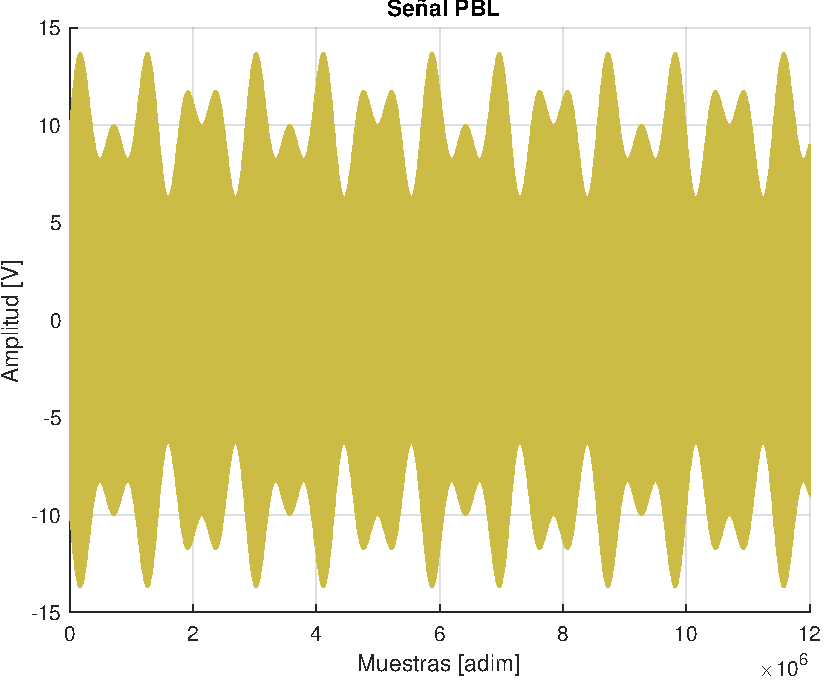
\includegraphics[width=0.45\linewidth]{include//figures/pbl.pdf}
    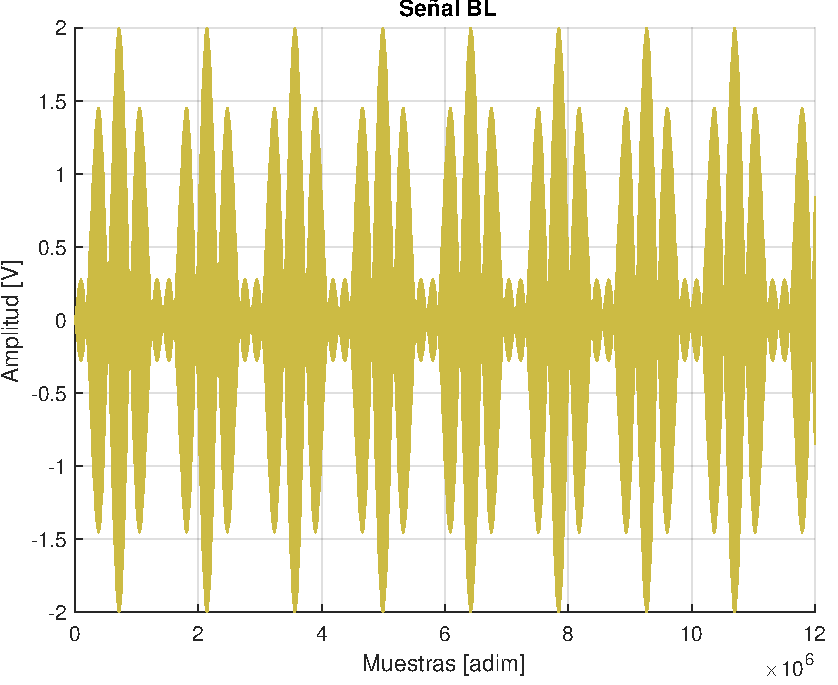
\includegraphics[width=0.45\linewidth]{include//figures/bl.pdf}
    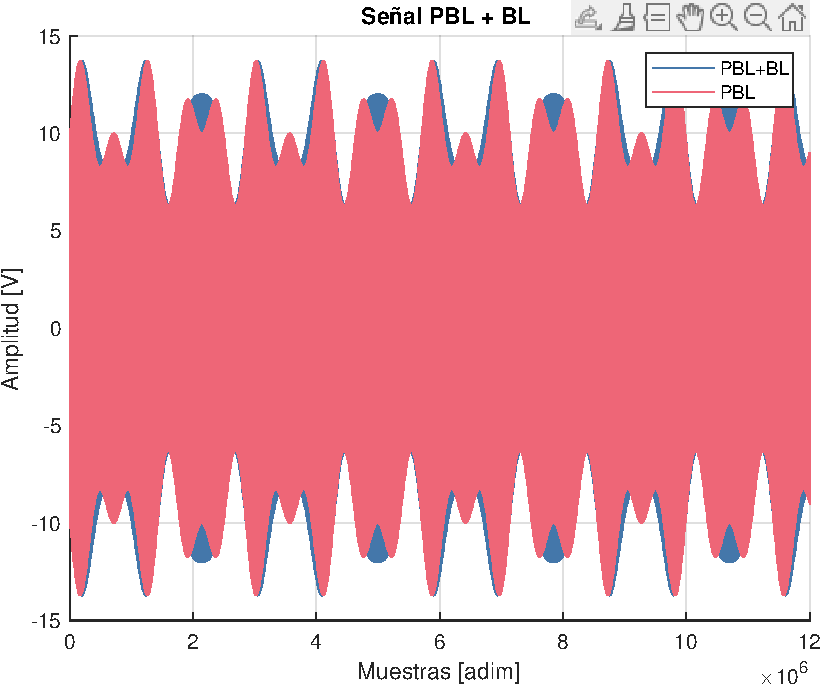
\includegraphics[width=0.5\linewidth]{include//figures/pbl+bl.pdf}
    \caption{Señal PBl (1), BL (2) y ambas (3)}
\end{figure}

\begin{figure}[!htb]
    \centering
    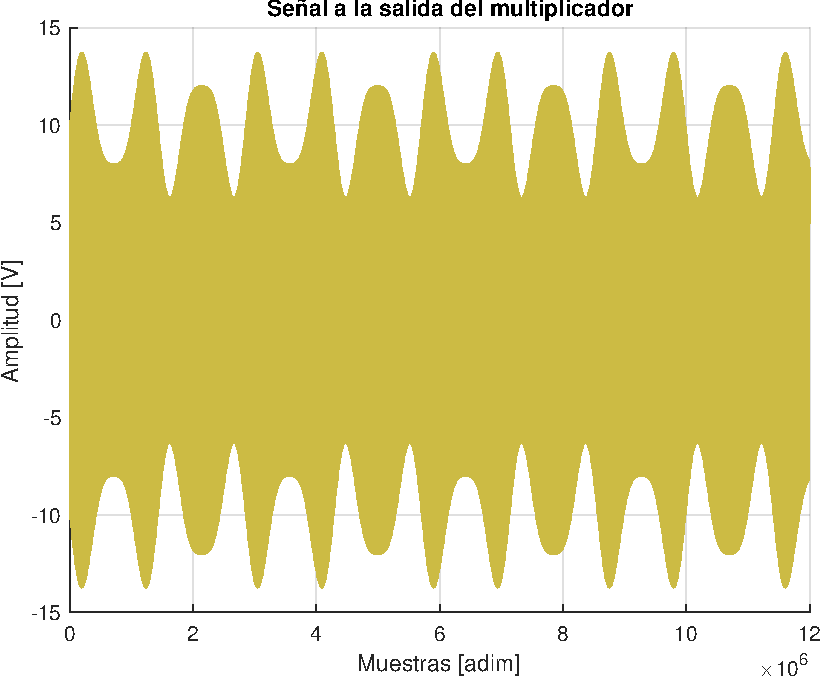
\includegraphics[width=0.45\linewidth]{include//figures/multiplicador.pdf}
    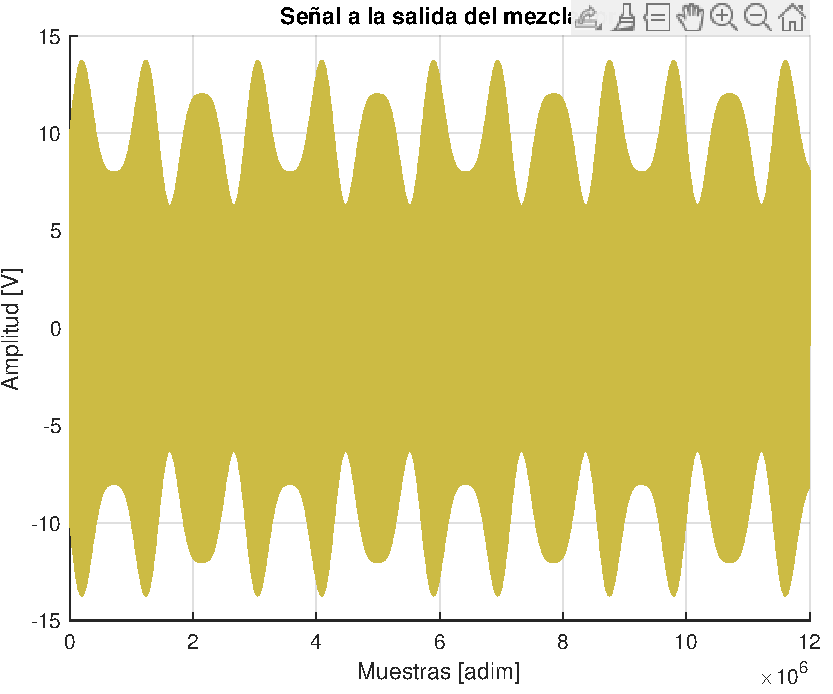
\includegraphics[width=0.45\linewidth]{include//figures/mezclador.pdf}
    \caption{Señal a la salida del mutliplicador (4) y del mezclador (5)}
\end{figure}


\begin{figure}[!htb]
    \centering
    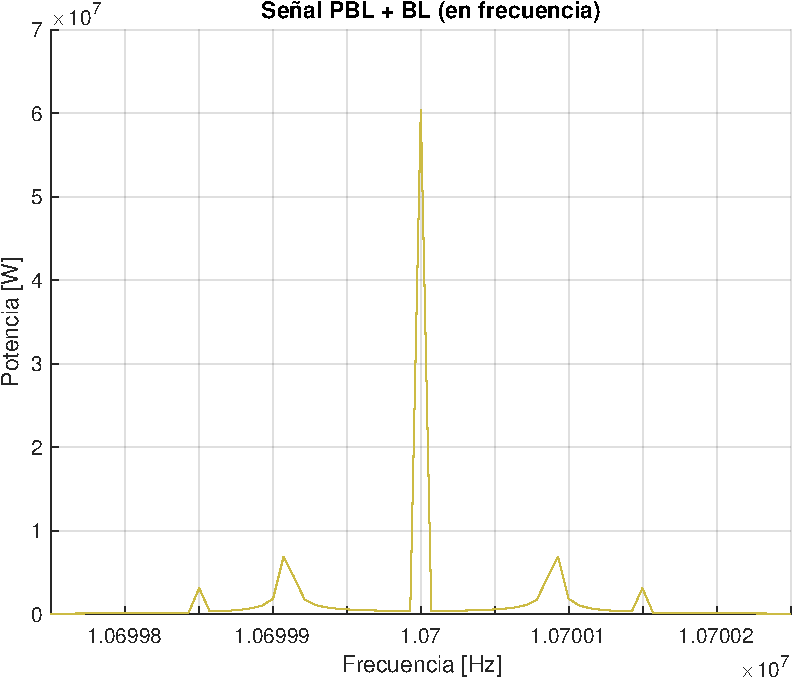
\includegraphics[width=0.45\linewidth]{include//figures/pbl+blhz.pdf}
    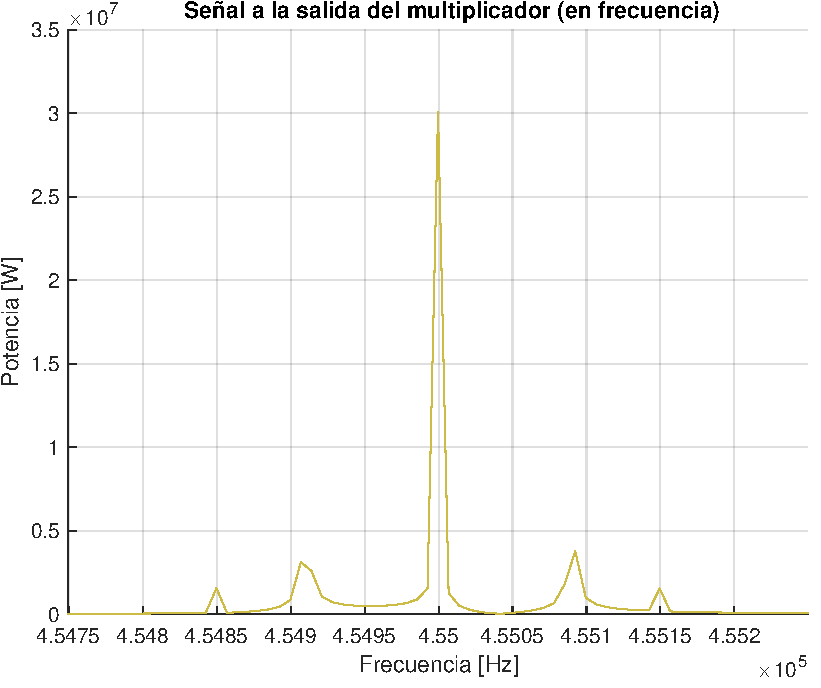
\includegraphics[width=0.45\linewidth]{include//figures/multiplicadorhz.pdf}
    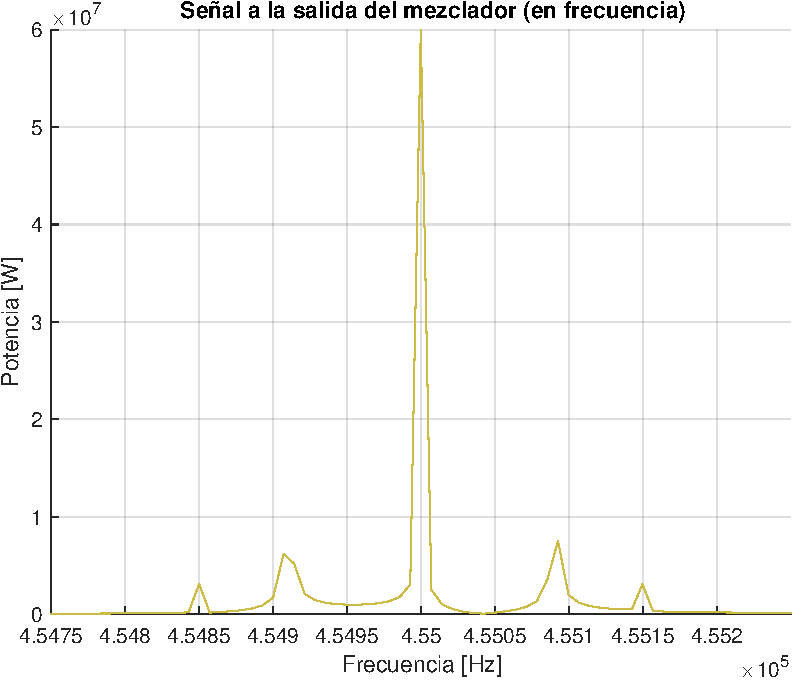
\includegraphics[width=0.5\linewidth]{include//figures/muestreo.pdf}
    \caption{Respuestas en frecuencia de PBL+BL, a la salida del mutliplicador y a la salida del mezclador (6)} 
\end{figure}


\begin{figure}[!htb]
    \centering
    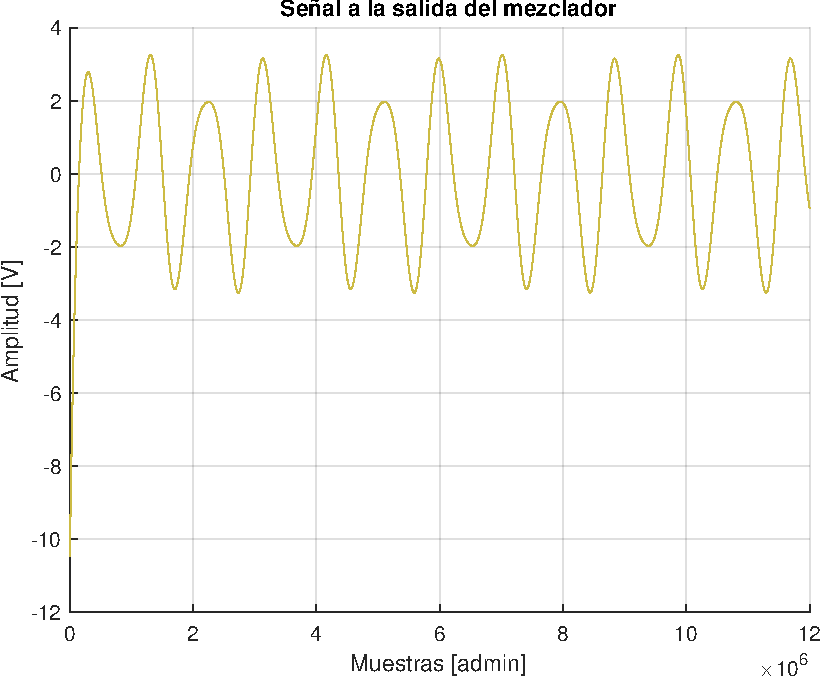
\includegraphics[width=0.6\linewidth]{include//figures/detector.pdf}
    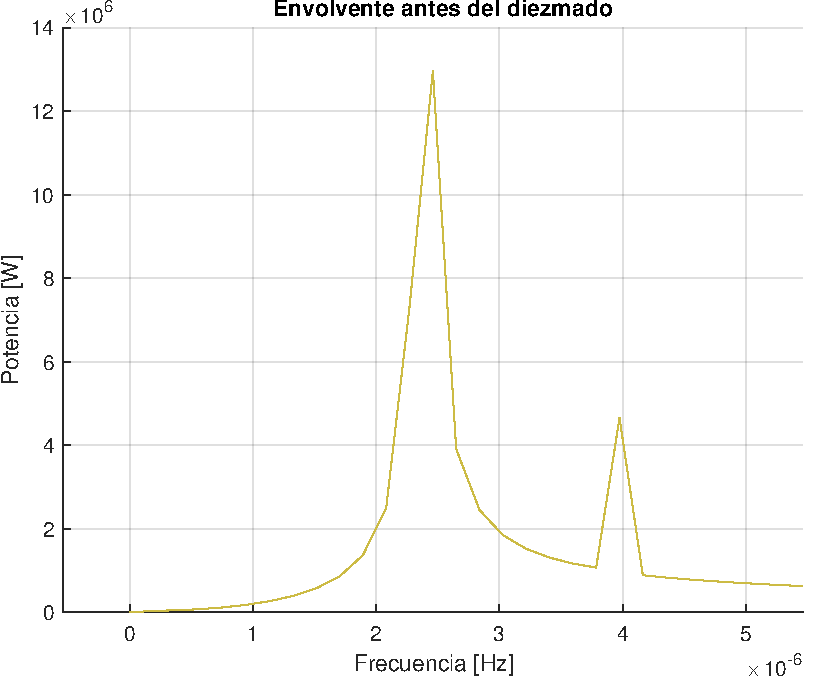
\includegraphics[width=0.45\linewidth]{include//figures/envolvente_antes.pdf}
    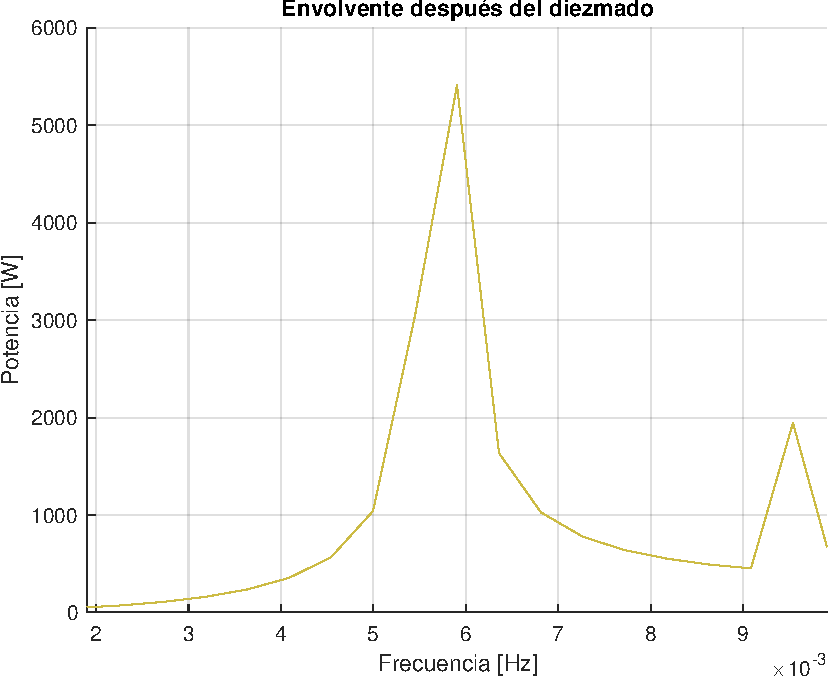
\includegraphics[width=0.45\linewidth]{include//figures/envolvente_despues.pdf}
    \caption{Señal a la salida del detector (7), espectro de la envolvente antes del diezmado y después (8)} 
\end{figure}


\begin{figure}[!htb]
    \centering
    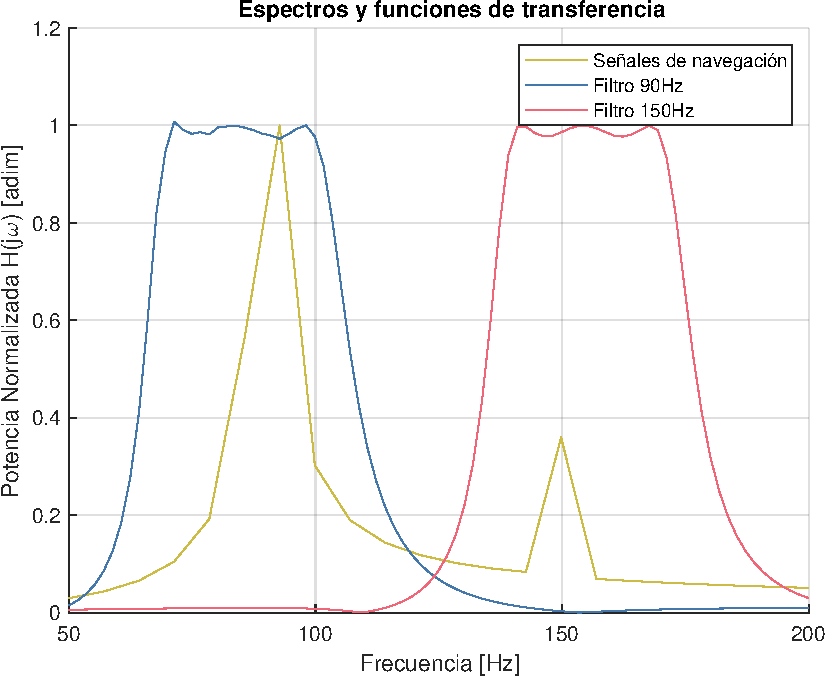
\includegraphics[width=0.45\linewidth]{include//figures/espectro.pdf}
    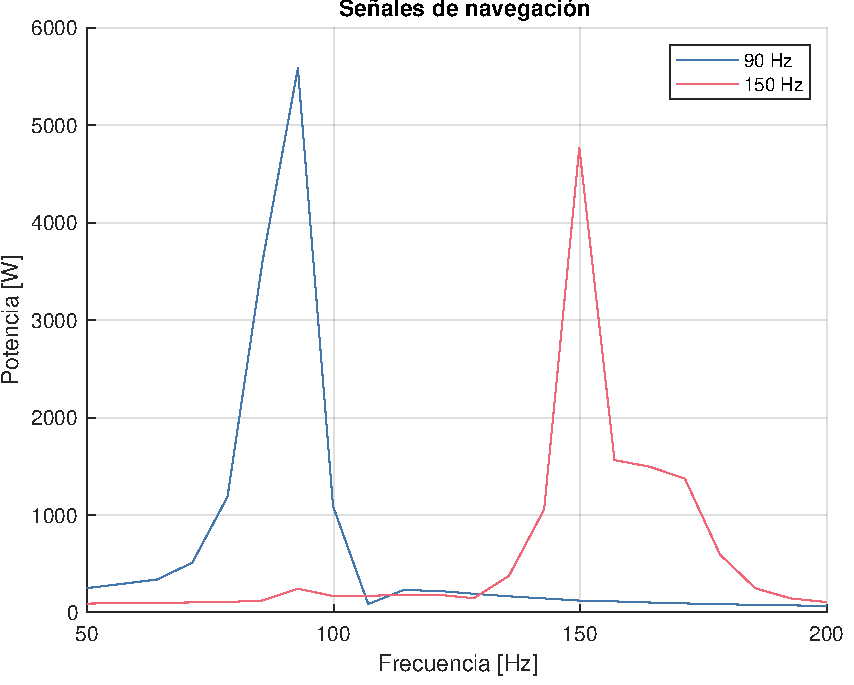
\includegraphics[width=0.45\linewidth]{include//figures/senales.pdf}
    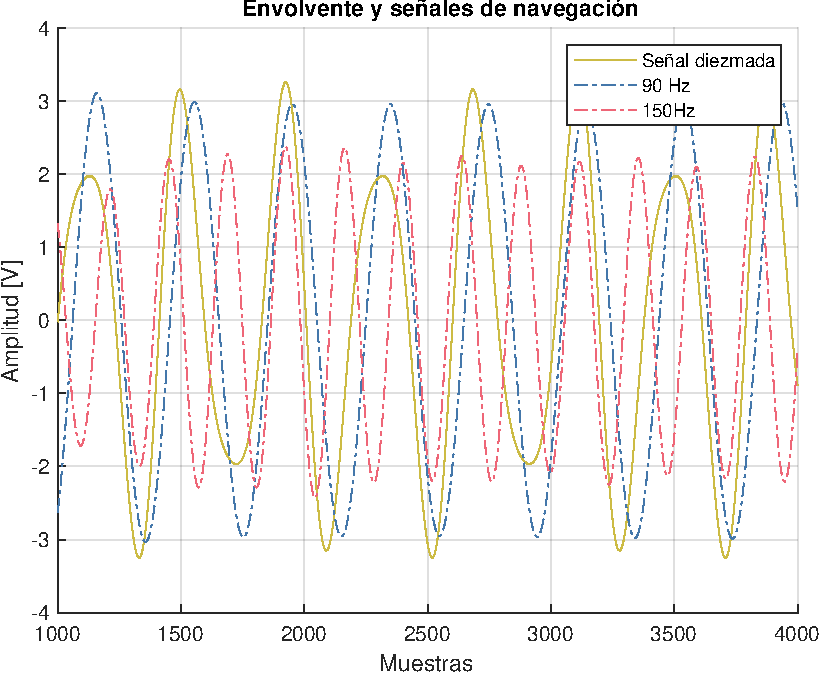
\includegraphics[width=0.6\linewidth]{include//figures/envolvente+senales.pdf}
    \caption{Espectro junto con módulo de las funciones de transferencia (9), señales de navegación y envolvente y señales de navegación (10)} 
\end{figure}




\section*{Código}
\lstset{inputencoding=utf8/latin1}
\lstinputlisting[
frame=single,
numbers=left,
style=Matlab-editor
]{Practica2425.m}


% ============
\end{document}